% This is samplepaper.tex, a sample chapter demonstrating the
% LLNCS macro package for Springer Computer Science proceedings;
% Version 2.20 of 2017/10/04
%
\RequirePackage{amsmath}
\documentclass[runningheads]{llncs}
%
%This is a template for producing LIPIcs articles. 
%See lipics-manual.pdf for further information.
%for A4 paper format use option "a4paper", for US-letter use option "letterpaper"
%for british hyphenation rules use option "UKenglish", for american hyphenation rules use option "USenglish"
%for section-numbered lemmas etc., use "numberwithinsect"
%for enabling cleveref support, use "cleveref"
%for enabling cleveref support, use "autoref"


% \bibliographystyle{plainurl}% the mandatory bibstyle

\usepackage{mathtools,mathpartir}
\usepackage{extarrows}
\usepackage{stmaryrd}
\usepackage{graphicx}
\usepackage{algorithm}
\usepackage[noend]{algpseudocode}
\usepackage{amsmath}
\usepackage{amssymb}
\usepackage{latexsym}
\usepackage{amstext}
\usepackage{xspace}
\usepackage{enumerate}
\usepackage{macrosLLNCS}
\usepackage{graphicx}
\usepackage{color}
\usepackage{epstopdf}
\usepackage{hyperref}
\usepackage{mathrsfs}
\hypersetup{
    colorlinks=true,
    linkcolor=black,
    filecolor=black,      
    urlcolor=blue,
    citecolor=black
}
% New definitions

\def\leaveout#1{}
\def\>{\ensuremath{\rangle}}
\def\<{\ensuremath{\langle}}
\def\h{\ensuremath{\mathcal{H}}}
\def\p{\ensuremath{\mathcal{P}}}
\def\l{\ensuremath{\mathcal{L}}}
\def\g{\ensuremath{\mathcal{G}}}
\def\lh{\ensuremath{\mathcal{L(H)}}}
\def\dh{\ensuremath{\mathcal{D(H})}}

\def\r{\ensuremath{\mathcal{R}}}

\def\ra{\ensuremath{\rightarrow}}
\def\e{\ensuremath{\mathcal{E}}}
\def\f{\ensuremath{\mathcal{F}}}

\def\c{\ensuremath{\mathcal{C}}}
\def\d{\ensuremath{\mathcal{D}}}
\def\le{\ensuremath{\sqsubseteq}}
\def\z{\ensuremath{{\bf 0}}}

\newcommand{\abis}{\stackrel{\lambda}\approx}
\newcommand{\abisa}[1]{\stackrel{#1}\approx}
\newcommand {\qbit} {\mbox{\bf{new}}}
\newcommand {\nil} {\mbox{\bf{nil}}}
\newcommand {\iif} {\mbox{\bf{if}}}
\newcommand {\then} {\mbox{\bf{then}}}
\newcommand {\eelse} {\mbox{\bf{else}}}
\newcommand {\qcf}[1] {{\sf{#1}}}
\newcommand{\con}[3]{\iif\ {#1}\ \then\ {#2}\ \eelse\ {#3}}

\newcommand{\ptr}{{\rm env}}
\newcommand{\rto}[1]{\stackrel{#1}\longrightarrow}
\newcommand{\Rto}[1]{\stackrel{#1}\Longrightarrow}
\newcommand{\nrto}[1]{\stackrel{#1}\nrightarrow}

\newcommand{\Rhto}[1]{\stackrel{\widehat{#1}}\Longrightarrow}
\newcommand{\define}{\stackrel{\it def}=}
\newcommand{\rsim}{\simeq}
\newcommand{\obis}{\approx_o}
%%%%%%%%%%%%%%%%% Distributions
\newcommand{\eDis}{\varepsilon}
\newcommand{\Stop}{{\times}}
\newcommand{\Mass}[1]{|#1|}
\newcommand{\subdist}[1]{\mathop{\mbox{$\mathcal D_{\textsl{sub}}$}}(#1)}
\newcommand{\dist}[1]{\mathop{Dist} ({#1})   } % distributions
\newcommand{\pdist}[1]{\overline{#1}  } % distributions
\newcommand{\support}[1]{\lceil{#1}\rceil}
\newcommand{\lift}[1]{\mathrel{{#1}^\circ}}

%%%%%%%%%%%%%%%% language
\newcommand{\probc}[1]{\mathrel{\!_{\scriptscriptstyle #1}\oplus}}
\newcommand{\Act}{\ensuremath{\mathsf{Act}}\xspace}

\newcommand{\setof}[2]{\{ \, #1 \, \mid \, #2 \, \}}% set comprehension
\newcommand{\Nat}{\mathbb{N}}
\newcommand{\Real}{\mathbb{R}}
\newcommand{\pair}[1]{\langle{#1}\rangle}
\newcommand{\ket}[1]{|{#1}\rangle}
\newcommand{\bra}[1]{\langle{#1}|}

%\newcommand{\so}{{\cal TSO}}
\newcommand{\Con}{{\it Con}}
\newcommand{\qv}{{\it qv}}
\newcommand{\qc}{\underline{c}}
\newcommand{\qd}{\underline{d}}
\newcommand{\cVar}{{\it cVar}}
\newcommand{\qVar}{{\it qVar}}
\newcommand{\cChan}{{\it cChan}}
\newcommand{\qChan}{{\it qChan}}
\newcommand{\tr}{{\rm tr}}
\newcommand{\CE}{{\cal E}}
\newcommand{\CH}{{\cal H}}
\newcommand{\CL}{{\cal L}}
\newcommand{\CC}{{\cal C}}
\newcommand{\CD}{{\cal D}}
\newcommand{\ifthen}[2]{{\textbf{if} ~#1~ \textbf{then} ~#2}}

\algnewcommand\algorithmicswitch{\textbf{switch}}
\algnewcommand\algorithmiccase{\textbf{case}}
\algnewcommand\algorithmicotherwise{\textbf{otherwise}}
\algnewcommand\algorithmicassert{\texttt{assert}}
\algnewcommand\Assert[1]{\State \algorithmicassert(#1)}%
% New "environments"
\algdef{SE}[SWITCH]{Switch}{EndSwitch}[1]{\algorithmicswitch\ #1\ \algorithmicdo}{\algorithmicend\ \algorithmicswitch}%
\algdef{SE}[CASE]{Case}{EndCase}[1]{\algorithmiccase\ #1}{\algorithmicend\ \algorithmiccase}%
\algdef{SE}[CASE]{Otherwise}{EndOtherwise}[1]{\algorithmicotherwise\ #1}{\algorithmicend\ \algorithmicotherwise}%
\algtext*{EndSwitch}%
\algtext*{EndCase}%
\algtext*{EndOtherwise}%
\usepackage{tabularx}
\usepackage{array}
\newcommand{\tabincell}[2]{\begin{tabular}{@{}#1@{}}#2\end{tabular}}

% New "environments"
\algdef{SE}[SWITCH]{Switch}{EndSwitch}[1]{\algorithmicswitch\ #1\ \algorithmicdo}{\algorithmicend\ \algorithmicswitch}%
\algdef{SE}[CASE]{Case}{EndCase}[1]{\algorithmiccase\ #1}{\algorithmicend\ \algorithmiccase}%
\algdef{SE}[CASE]{Otherwise}{EndOtherwise}[1]{\algorithmicotherwise\ #1}{\algorithmicend\ \algorithmicotherwise}%
\algtext*{EndSwitch}%
\algtext*{EndCase}%
\algtext*{EndOtherwise}%
\usepackage{tabularx}
\usepackage{array}
%\newcommand{\tabincell}[2]{\begin{tabular}{@{}#1@{}}#2\end{tabular}}

\makeatletter
\newenvironment{breakablealgorithm}
  {% \begin{breakablealgorithm}
   \begin{center}
     \refstepcounter{algorithm}% New algorithm
     \hrule height.8pt depth0pt \kern2pt% \@fs@pre for \@fs@ruled
     \renewcommand{\caption}[2][\relax]{% Make a new \caption
       {\raggedright\textbf{\ALG@name~\thealgorithm} ##2\par}%
       \ifx\relax##1\relax % #1 is \relax
         \addcontentsline{loa}{algorithm}{\protect\numberline{\thealgorithm}##2}%
       \else % #1 is not \relax
         \addcontentsline{loa}{algorithm}{\protect\numberline{\thealgorithm}##1}%
       \fi
       \kern2pt\hrule\kern2pt
     }
  }{% \end{breakablealgorithm}
     \kern2pt\hrule\relax% \@fs@post for \@fs@ruled
   \end{center}
  }
\makeatother

% Long table
\usepackage{longtable}
\usepackage{multirow}

% Text color
\newcommand{\QIN}[1]{\textcolor{blue}{#1}}

% Used for displaying a sample figure. If possible, figure files should
% be included in EPS format.
%
% If you use the hyperref package, please uncomment the following line
% to display URLs in blue roman font according to Springer's eBook style:
% \renewcommand\UrlFont{\color{blue}\rmfamily}

\begin{document}
%
\title{Verifying Quantum Communication Protocols with Distribution-based Bisimulation}
%
%\titlerunning{Abbreviated paper title}
% If the paper title is too long for the running head, you can set
% an abbreviated paper title here
%
\author{Xudong Qin\inst{1,2}\and
Yuxin Deng\inst{1,2} \and 
Yuan Feng}
%
\authorrunning{X. Qin \and
Y. Deng \and 
Y. Feng}
% First names are abbreviated in the running head.
% If there are more than two authors, 'et al.' is used.
%
\institute{Shanghai Key Laboratory of Trustworthy Computing\and East China Normal University, China\and
XXXXXXX}
%
\maketitle              % typeset the header of the contribution
%
\begin{abstract}
The process algebra is one of the useful techniques in formal verification. It has been extended to several quantum versions for describing quantum communication protocols in a number of works. Bisimulation presents the behavioural equivalence between processes through process algebra. It enables us to check whether an implementation of a protocol is consistent with its specification. Considering the quantum state depends on the history of the quantum operations applied on it, we give a distribution-based quantum ground bisimulation which is more suitable to present the equivalence between quantum operations. We also implement a algorithm to check if two given quantum processes are distribution-based ground bisimilar and then we make the experiments on several interesting quantum protocols so that we can compare it with the checking algorithm of the state-based bisimulation.

\keywords{Quantum process algebra \and Bisimulation \and
Verification \and Quantum communication protocols.}
\end{abstract}
%
%
%
\section{Introduction}
Quantum mechanical principles such as non-cloning property and entanglement have been used in a number of previous works to design quantum communication protocols which are more efficient and secure ranging from the teleportation protocol~\cite{BB93} to key distribution protocols like BB84~\cite{BB84} and B92~\cite{B92}. It brings difficulty to verify the correctness of the quantum protocols as the general quantum computer is still under developing. Formal methods are introduced to check the protocols at the design stage. 

Process algebra is one of the useful techniques in the formal method providing the specification and verification of communicating and concurrent systems. 
Their extensions to the quantum setting have already appeared in the literature. Jorrand and Lalire \cite{JL04,La06} defined the \emph{Quantum Process Algebra} (QPAlg) and presented a branching bisimulation to identify quantum processes with the same branching structure. Gay and Nagarajan~\cite{GN05}  developed \emph{Communicating Quantum Processes} (CQP), for which Davidson~\cite{Da11} established a bisimulation congruence.
Feng et al. \cite{FDJY07} have proposed a quantum variant of classical value-passing CCS \cite{ccs}, called qCCS, and a notion of probabilistic bisimulation for quantum processes, which is then improved to be a general notion of bisimulation that enjoys a congruence property \cite{FDY11}. Later on, motivated by~\cite{San96}, Deng and Feng~\cite{DF12} defined an open bisimulation for quantum processes that makes it possible to separate ground bisimulation and the closedness under super-operator applications, thus providing not only a neater and simpler definition, but also a new technique for proving bisimilarity.
In order to avoid the problem of instantiating quantum variables by potentially infinitely many quantum states, Feng et al.~\cite{FDY14} extended the idea of symbolic bisimulation~\cite{HL95} for value-passing CCS and provided a symbolic version of open bisimulation for qCCS. They  proposed an algorithm for checking symbolic ground bisimulation.

In the current work, we consider a distribution-based ground bisimulation rather than the state-based ground bisimualtion proposed in \cite{DF12}. The processes are encoded in qCCS with fixed initial quantum states. We compute a bisimulation matrix to check if two process are bisimilar. The algorithm extends the general distribution-based bisimulation checking method in~\cite{HKK14} taking the check on the quantum states into account. 

The definition the distribution-based ground bisimulation is based on the definition of the state-based ground bisimulation proposed in~\cite{DF12}, changing the transition from a state to a distribution of states into the transition between distributions. It is already known that for any convex and continuous equivalence relation there exists a characteristic matrix for it which can check if two distributions satisfy the relation. As the  distribution-based quantum ground bisimulation is also a convex and continuous equivalence relation, we can compute its characteristic matrix, called bisimulation matrix, for bisimilarity checking. 
We have developed a tool that implements the algorithm and check if two given bisimulations are strongly or weakly bisimilar. Then we have conducted experiments on a few interesting quantum communication protocols including super-dense coding, teleportation, secret sharing, and several quantum key distribution protocols. We also have made a comparison between the distribution-based version and state-based version of bisimilarity checking algorithms.

\paragraph{Other related work} In the equivalence checking for the quantum processes, Ardeshir-Larijani et al.~\cite{AL18} proposed a quantum variant of CCS called Quantum Programming Language (QPL)~\cite{Sel04}, to describe quantum protocols. The syntax of that variant is similar to qCCS but its semantics is very different. The behaviour of a concurrent process is described as a finite tree and an interleaving is a path from the root to a leaf. By interpreting an interleaving as a superoperator, the semantics of a process is a set of superoperators. Then they introduce the stabiliser simulation algorithm invented by Aaronson and Gottesman~\cite{AG04} for the equivalence checking between two processes.
Ardeshir-Larijani et al. have implemented their approach in an automated equivalence checker in Java and verified several quantum protocols from teleportation to secret sharing. However the input of the states are limited to the stabilizer states.

Kubota et al.~\cite{KKKKS16} implemented a semi-automated tool to check a notion of symbolic bisimulation and used it to verify the equivalence of BB84 and another quantum key distribution protocol based on entanglement distillation \cite{SP00}. The checking algorithm is based on the equational reasoning in which users need to provide equations during the checking procedure thus it is semi-automated.

The the distribution-based weak bisimulations has been introduced in~\cite{ehz}. After that several works distribution-based bisimulations have been proposed. A decision algorithm for the weak bisimulation of the probabilistic automata is proposed in~\cite{EHKT13}. Then a general and natural notion of the distribution-based bisimulation is given in~\cite{HKK14} together with algorithms for computing such bisimulation relation in both finite and a part of infinite systems. Motivated by the unrealistic requirement of the current general scheduler on distributed systems, Zhang et al.~\cite{ZYSHEJG18} have proposed a coarser weak bisimilarity called late distribution bisimilarity.

The rest of the paper is structured as follows.
In Section~\ref{sec:qccs} we recall the syntax and semantics of the quantum process algebra qCCS. In Section~\ref{sec:distribution-based bisimulation} we define a distribution-based quantum ground bisimulations and show the relation between the state-based version and distribution-based version. In Section~\ref{sec:distribution-based bisimulation algorithm}  we present an algorithm for checking distribution-based ground bisimulation. In Section~\ref{sec:weak} we extend the method to check the weak distribution-based ground bisimulation which abstract invisible actions away. In Section~\ref{sec:weak_experiment} we report some experimental results on verifying a few quantum communication protocols and make a comparison with the state-based version of the bisimulation checking algorithm. Finally, we conclude in Section~\ref{sec:conclusion} and discuss some future work.

\section{Preliminary}
\label{sec:qccs}
We introduce a quantum extension of classical CCS (qCCS) which was originally studied in \cite{FDJY07,YFDJ09,FDY11}. Three types of data are considered in qCCS: as classical data we have \texttt{Bool} for booleans and \texttt{Real} for real numbers, and as quantum data we have \texttt{Qbt} for qubits. Consequently,
two countably infinite sets of variables are assumed: $\cVar$ for classical variables, ranged over by $x,y,...$, and $\qVar$ for quantum variables, ranged over by $q,r,...$.
We assume a set ${\it Exp}$, which includes $\cVar$ as a subset and is ranged over by $e,e',\dots$,  of classical data expressions over
\texttt{Real}, and a set of boolean-valued expressions ${\it BExp}$, ranged over by $b, b',\dots$, with the usual boolean constants $\texttt{true}$, $\texttt{false}$, and operators
$\neg$, $\wedge$, $\vee$, and $\ra$. In particular, we let $e\bowtie e'$ be a boolean expression for any $e,e'\in {\it Exp}$ and ${\bowtie} \in\sset{>, <, \geq, \leq, =}$.
We further assume that only classical variables can occur freely in both data expressions and boolean expressions.
Two types of channels are used: $\cChan$ for classical channels, ranged over by $c,d,...$, and $\qChan$ for quantum channels, ranged over by $\qc,\qd$,.... A relabelling function $f$ is a map on $\cChan\; \cup\; \qChan$ such that $f(\cChan)\subseteq \cChan$ and $f(\qChan)\subseteq \qChan$.
Sometimes we abbreviate a sequence of distinct variables $q_1,...,q_n$ into $\tilde{q}$.

The terms in qCCS are given by:
\[\begin{array}{rcl}
P,Q &::=& \Cnil \BNFsep \tau.P \BNFsep c?x.P \BNFsep c!e.P
\BNFsep \qc?q.P \BNFsep
\qc!q.P \BNFsep \CE[\tilde{q}].P
\BNFsep M[\tilde{q};x].P \BNFsep \\
& & P + Q \BNFsep  P \Cpar Q\;
\BNFsep P[f] \BNFsep P\backslash L \BNFsep \ifthen{b}{P} \BNFsep
A(\tilde{q};\tilde{x})
\end{array}\]
where $f$ is a relabelling function and $L\subseteq \cChan\cup \qChan$ is a set of channels.
Most of the constructors are standard as in CCS \cite{ccs}.
We briefly explain a few new constructors. The process $\qc?q.P$ receives a quantum datum along quantum channel $\qc$ and evolves into $P$, while $\qc!q.P$ sends out a quantum datum along quantum channel $\qc$ before evolving into $P$. The symbol $\CE$ represents a trace-preserving super-operator applied on the systems $\tilde{q}$. The process $M[\tilde{q};x].P$ measures the state of qubits $\tilde{q}$
according to the observable $M$ and stores the measurement outcome into the
classical variable $x$ of $P$.

Free classical variables can be defined in the usual way, except for the fact that the variable $x$ in the quantum measurement $M[\tilde{q};x]$ is bound. A process $P$ is closed if it contains no free classical variable, i.e. $fv(P)=\emptyset$.

The set of free quantum variables for process $P$, denoted by $qv(P)$ can be inductively defined as in Figure~\ref{fig:fqv}.
\begin{figure*}[t]
	\[\small\begin{array}{rclrcl}
	qv(\Cnil) & = & \emptyset & qv(\tau.P) & = & qv(P)\\
	qv(c?x.P) & = & qv(P) & qv(c!e.P) & = & qv(P) \\
	qv(\qc?q.P) & = & qv(P)-\sset{q} & qv(\qc!q.P) & = & qv(P)\cup\sset{q} \\
	qv(\CE[\tilde{q}].P) & = & qv(P)\cup \tilde{q} &
	qv(M[\tilde{q};x].P) & = & qv(P) \cup \tilde{q}\\
	qv(P+Q) & = & qv(P)\cup qv(Q) \qquad &
	qv(P \Cpar Q) & = & qv(P)\cup qv(Q)\\
	qv(P[f]) & = & qv(P) &
	qv(P\backslash L) & = & qv(P)\\
	qv(\ifthen{b}{P}) & = & qv(P) &
	qv(A(\tilde{q};\tilde{x})) & = & \tilde{q}.
	\end{array}\]
	\caption{Free quantum variables}\label{fig:fqv}
\end{figure*}
For a process to be legal, we require that
\begin{enumerate}
	\item $q\not\in qv(P)$ in the process $\qc!q.P$;
	\item $qv(P)\cap qv(Q)=\emptyset$ in the process $P \Cpar Q$;
	\item Each constant $A(\tilde{q};\tilde{x})$ has a defining equation $A(\tilde{q};\tilde{x}) \Defs P$, where $P$ is a term with $qv(P)\subseteq\tilde{q}$ and $fv(P)\subseteq \tilde{x}$.
\end{enumerate}
The first condition says that a quantum system will not be referenced after it has been sent out. This is a requirement of the quantum no-cloning theorem. The second condition says that parallel composition $\Cpar$ models separate parties that never reference a quantum system simultaneously. 

\begin{figure*}[t]
	\[\small\begin{array}{ll}
	\slinfer[\Rlts{Tau}]{\pair{\tau.P, \rho} \ar{\tau} \pair{P, \rho}}
	&\linfer[\Rlts{C-Inp}]{v\in\texttt{Real}}{\pair{c?x.P,\rho} \ar{c?v} \pair{P[v/x],\rho}}
	\\[3pt]
	\linfer[\Rlts{C-Outp}]{v=\Op{e}}{\pair{c!e.P,\rho} \ar{c!v} \pair{P,\rho} }
	
	&
	\linfer[\Rlts{C-Com}]{\pair{P_1,\rho}\ar{c?v}\pair{P'_1,\rho}\qquad
		\pair{P_2,\rho}\ar{c!v}\pair{P'_2,\rho}
	}
	{\pair{P_1\Cpar P_2,\rho} \ar{\tau} \pair{P'_1\Cpar P'_2,\rho} }
	\\[3pt]
	\linfer[\Rlts{Q-inp}]{r\not\in qv(\qc?q.P)}
	{\pair{\qc?q.P,\rho} \ar{\qc?r} \pair{P[r/q],\rho}}
	&
	\slinfer[\Rlts{Q-Outp}]{\pair{\qc!q.P,\rho} \ar{\qc!q} \pair{P,\rho} }
	\\[3pt]
	\linfer[\Rlts{Q-Com}]{\pair{P_1,\rho} \ar{\qc?r} \pair{P'_1,\rho} \qquad \pair{P_2,\rho}\ar{\qc!r} \pair{P'_2,\rho}}
	{\pair{P_1\Cpar P_2, \rho } \ar{\tau} \pair{P'_1\Cpar P'_2, \rho}}
	&
	\slinfer[\Rlts{Oper}]{\pair{\CE[\tilde{q}].P,\rho} \ar{\tau} \pair{P,\CE_{\tilde{q}}(\rho)}}
	\\[3pt]
	\linfer[\Rlts{Meas}]{M=\sum_{i\in I}\lambda_i E^i \qquad p_i=tr(E^i_{\tilde{q}}\rho)}
	{\pair{M[\tilde{q};x].P,\rho} \ar{\tau} \sum_{i\in I}p_i \pair{P[\lambda_i/x], E^i_{\tilde{q}}\rho E^i_{\tilde{q}} / p_i}}
	&
	\\
	\linfer[\Rlts{Int}]{\pair{P_1,\rho} \ar{\alpha} \Delta\qquad qbv(\alpha)\cap qv(P_2)=\emptyset}{\pair{P_1 \Cpar P_2,\rho} \ar{\alpha} \Delta\Cpar P_2}
	%\\[3pt]
	%\linfer[\Rlts{Inp-Int}]{\pair{P_1,\rho} \ar{\qc?r} \pair{P'_1,\rho}\qquad r\not\in qv(P_2)}{\pair{P_1\Cpar P_2,\rho} \ar{\qc?r} \pair{P'_1\Cpar P_2,\rho}}
	&
	\linfer[\Rlts{Sum}]{\pair{P_1,\rho} \ar{\alpha} \Delta}{\pair{P_1+P_2,\rho} \ar{\alpha} \Delta}
	\\[3pt]
	\linfer[\Rlts{Rel}]{\pair{P,\rho} \ar{\alpha} \Delta}{\pair{P[f],\rho} \ar{f(\alpha)} \Delta[f]}
	&
	\linfer[\Rlts{Res}]{\pair{P,\rho} \ar{\alpha} \Delta \qquad cn(\alpha)\cap L=\emptyset}{\pair{P\backslash L,\rho} \ar{\alpha} \Delta\backslash L}
	\\[3pt]
	\linfer[\Rlts{Cho}]{\pair{P,\rho} \ar{\alpha} \Delta \qquad \Op{b}=\texttt{true}}{\pair{\ifthen{b}{P},\rho} \ar{\alpha} \Delta}
	&
	\linfer[\Rlts{Cons}]{\pair{P[\tilde{v}/\tilde{x},\tilde{r}/\tilde{q}],\rho} \ar{\alpha} \Delta \qquad A(\widetilde{x}, \tilde{q})\Defs P}{\pair{A(\tilde{v},\tilde{r}),\rho} \ar{\alpha} \Delta}
	\end{array}\]
	\caption{Operational semantics of qCCS. Here in rule $\Rlts{C-Outp}$, $\Op{e}$ is the evaluation of $e$, and in rule $\Rlts{Meas}$, $E^i_{\tilde{q}}$ denotes the operator $E^i$ acting on the quantum systems $\tilde{q}$.\label{fig:opsem}
	}
\end{figure*}

Throughout the paper we implicitly assume the convention that processes are identified up to $\alpha$-conversion, bound variables differ from each other and they are different from free variables.

We also give the semantics of qCCS. We start at the definition of probabilistic labelled transition systems (pLTSs) by which we present the behavior of the quantum processes. We first introduce the notation of the probability distribution. A discrete probability distribution over a set $S$ is a function $\Delta: S\rightarrow [0,1]$ with $\sum_{s\in S} \Delta(s) = 1$ and the support of the distribution $\Delta$ is the set $\lceil\Delta\rceil = \{s\in S|\Delta(s)>0\}$. The point distribution $\overline{s}$ assigns probability $1$ to the element $s$ and $0$ to all other elements of $S$, so that $\lceil\overline{s}\rceil = \{s\}$. The empty distribution $\epsilon$ assigns $0$ to all other elements of $S$ and $\lceil\epsilon\rceil = \emptyset$.

Let $S$ be the set of states and $Dist(S)$ be the probability distribution over $S$, ranged over by $\Delta$, $\Theta$, etc. The probabilistic labelled transition system can be defined as follow.

\begin{definition}\label{def:pLTS}
A probabilistic labelled transition system (pLTS) is a tuple $P=\langle S,Act_{\tau},\xrightarrow{}\rangle$ where $\xrightarrow{}\in S\times Dist(S)$ is the smallest relation satisfying:
\begin{itemize}
    \item if $s\xrightarrow{\alpha}\Delta$ then $\overline{s}\xrightarrow{\alpha}\Delta$;
    \item if $s\not\xrightarrow{\alpha}$ then $\overline{s}\xrightarrow{\alpha}\epsilon$;
    % \item if $\Delta_{i}\xrightarrow{\alpha}\Theta_{i}$ for each $i\in I$, then there exists $\sum_{i}p_{i}\Delta_{i}\xrightarrow{\alpha}\sum_{i}p_{i}\Theta_{i}$ where $I$ is a finite set and $\sum_{i}p_{i}=1\wedge p_{i}\geq 0$.
\end{itemize}
\end{definition}

The operational semantics of qCCS are given in Figure~\ref{fig:opsem}. For each quantum variable $q$ we assume a 2-dimensional Hilbert space $\CH_q$. For any nonempty subset $S\subseteq \qVar$ we write $\CH_S$ for the tensor product space $\bigotimes_{q\in S}\CH_q$ and $\CH_{\overline{S}}$ for $\bigotimes_{q\not\in S}\CH_q$. In particular, $\CH=\CH_{\qVar}$ is the state space of the whole environment consisting of all the quantum variables, which is a countably infinite dimensional Hilbert space.

Let $P$ be a closed quantum process and $\rho$ a density operator on $\CH$\footnote{As $\CH$ is infinite dimensional, $\rho$ should be understood as a density operator on some finite dimensional subspace of $\CH$ which contains $\h_{\qv(P)}$.}, the pair $\pair{P,\rho}$ is called a \emph{configuration}. We write $\Con$ for the set of all configurations, ranged over by $\CC$ and $\CD$. The trace of $\rho$ is defined as $tr(\rho)$.

We interpret qCCS with a pLTS whose states are all the configurations definable in the language, and whose transitions are determined by the rules in Figure~\ref{fig:opsem}; we have omitted the obvious symmetric counterparts to the rules \Rlts{C-Com}, \Rlts{Q-Com}, \Rlts{Int} and \Rlts{Sum}. The set of actions $\textbf{Act}$ takes the following form, consisting of classical/quantum input/output actions.

\begin{eqnarray*}
\textbf{Act} = 
	\sset{c?v, c!v \mid c\in \cChan, v\in\texttt{Real}}&\cup&
	\sset{\qc?r,\qc!r \mid \qc\in \qChan,r\in \qVar}
\end{eqnarray*}

%The symbol $\tau$ denotes invisible actions. We write $\Act$ for $\Act\cup\sset{\tau}$, which is ranged over by $\alpha$.
We use $cn(\alpha)$ for the set of channel names in action $\alpha$. For example, we have $cn(\qc?x)=\sset{\qc}$ and $cn(\tau)=\emptyset$.

In the first eight rules in Figure~\ref{fig:opsem}, the targets of arrows are point distributions, and we use the slightly abbreviated form $\CC\ar{\alpha}\CC'$ to mean $\CC\ar{\alpha}\pdist{\CC'}$.

The rules use the obvious extension of the function~$\Cpar$ on terms to configurations and distributions. To be precise,
$\CC\Cpar P$ is the configuration $\<Q\Cpar P,\rho \>$ where $\CC=\<Q,\rho\>$, and
$\Delta\Cpar P$ is the distribution defined by:
%\vskip -2mm
\[(\Delta\Cpar P)(\pair{Q,\rho}) \define \left\{\begin{array}{ll}
\Delta(\pair{Q',\rho}) & \mbox{if $Q=Q'\Cpar P$ for some } Q'\\
0 & \mbox{otherwise.}
\end{array}\right.\]
Similar extension applies to $\Delta[f]$ and $\Delta\backslash L$.

\section{Distribution-based Bisimulation}
\label{sec:distribution-based bisimulation}
We introduce the definition of the state-based bisimulation~\cite{DF12,FDY14} first. Here we still need to consider the relations between distributions, so we make the use of the lifting operation.

\begin{definition}\label{def:lift_rel}
Let $\aRel \in S\times S$ be a relation between states of pLTSs. We can lift $\aRel$ to $\lift{\aRel}\in Dist(S)\times Dist(S)$ which is the smallest relation satisfying:
\begin{itemize}
    \item $s\aRel s'$ implies that $\overline{s}\lift{\aRel} \overline{s'}$;
    \item $\Delta_{i}\lift{\aRel}\Theta_{i}$ for all $i\in I$ implies $(\sum_{i}p_{i}\Delta_{i})\lift{\aRel}(\sum_{i}p_{i}\Theta_{i})$ for any $p_{i}$ with $\sum_{i}p_{i}=1\wedge p_{i}\geq 0$,
\end{itemize}
where $I$ is a finite set of the distribution indices.
\end{definition}

We give the definition of the state-based bisimulation as follow. The notation $tr_{qv(P)}(\rho)$ is the partial trace over system $P$ at the configuration $\pair{P,\rho}$ whose result is a reduced density operator presenting the state of the environment.

\begin{definition}\label{def:state_strong_bisim}
\label{def:state-based strong ground bisimulation}
A state-based strong ground bisimulation is a symmetry relation $\aRel\in Con\times Con$ for any $\langle P,\rho\rangle, \langle Q,\sigma\rangle\in Con$ such that $\langle P,\rho\rangle\aRel\langle Q,\sigma\rangle$ implies
\begin{itemize}
    \item $qv(P)=qv(Q)$ and $tr_{qv(P)}(\rho)=tr_{qv(Q)}(\sigma)$;
    \item whenever $\langle P,\rho\rangle\xlongrightarrow{\alpha}\Delta'$, there exists $\Theta'$ such that $\langle Q,\sigma\rangle\xlongrightarrow{\alpha}\Theta'$ and $\Delta'\lift{\aRel}\Theta'$.
\end{itemize}
\end{definition}
We set $\langle P,\rho\rangle\sim\langle Q,\sigma\rangle$ if there is a strong ground bisimulation $\aRel$ such that $\langle P,\rho\rangle\aRel\langle Q,\sigma\rangle$.

If we take the history of the superoperator applied on $\rho$ into account, we should consider the transition between distributions instead of the transition from a single state to a distribution.

We change the transitions in pLTS into the transition between distributions. For the relation $\rightarrow\ \in Dist(S)\times Dist(S)$, we write $\Delta\xlongrightarrow{\alpha}\Theta$ where $\Theta=\sum\nolimits_{s\in\lceil\Delta\rceil}\Delta(s)\cdot\Delta_{s}$ and $s\xlongrightarrow{\alpha}\Delta_{s}$. After that, the distribution-based bisimulation is as follows.

\begin{definition}\label{def:dis_strong_bisim}
A distribution-based strong ground bisimulation is a symmetry relation $\aRel^{D}\in Dist(Con)\times Dist(Con)$ for any $\Delta,\Theta\in Dist(Con),\Delta=\sum_{i}p_{i}\langle t_{i},\rho_{i}\rangle,\Theta=\sum_{j}q_{j}\langle u_{j},\sigma_{j}\rangle$ such that $\Delta\aRel^{D}\Theta$ implies
\begin{itemize}
    \item $qv(\Delta)=qv(\Theta)$ and $\sum_{i}p_{i}tr_{qv(\Delta)}(\rho_{i})=\sum_{j}q_{j}tr_{qv(\Theta)}(\sigma_{j})$;
    \item whenever $\Delta\xlongrightarrow{\alpha}\Delta'$, there exists $\Theta'$ such that $\Theta\xlongrightarrow{\alpha}\Theta'$ and $\Delta'\aRel^{D}\Theta'$.
\end{itemize}
\end{definition}
We set $\Delta\sim_{D}\Theta$ if there is a strong ground bisimulation $\aRel^{D}$ such that $\Delta\aRel^{D}\Theta$.

Then we discuss the relation between the lifted state-based bismulation $\lift{\aRel}$ and the distribution-based bisimulation $\aRel^{D}$. For any $\aRel$, if there are $\Delta,\Theta\in Dist(Con)$ and $\Delta\lift{\aRel}\Theta$, we can take $\aRel^{D}=\lift{\aRel}$ and then there is $\Delta\aRel^{D}\Theta$. In the other direction, we consider the example in Fig.~\ref{fig:example}.

We take two distributions $\Delta, \Theta\in Dist(Con)$ where $\Delta=\frac{1}{2}s_1+\frac{1}{4}s_2+\frac{1}{4}s_3$ and $\Theta=\frac{1}{4}t_1+\frac{1}{4}t_2+\frac{1}{2}s_3$. There are transitions $\Delta\xrightarrow{}\Lambda$ and $\Theta\xrightarrow{}\Lambda$ where $\Lambda\in Dist(Con)$,  $\Lambda=\frac{1}{4}a+\frac{1}{4}b+\frac{1}{4}c+\frac{1}{4}d$.

Assume that the quantum variables used in each configuration of the pLTS are the same. Then we have $\Delta\aRel^{D} \Theta$ according to Definition~\ref{def:dis_strong_bisim}. Meanwhile, for each $s_{i}$, there is no $t_{i}$ such that $s_{i}\aRel t_{i}$, so $\Delta\lift{\aRel}\Theta$ cannot be satisfied.

\begin{figure}[htbp]
    \centering
    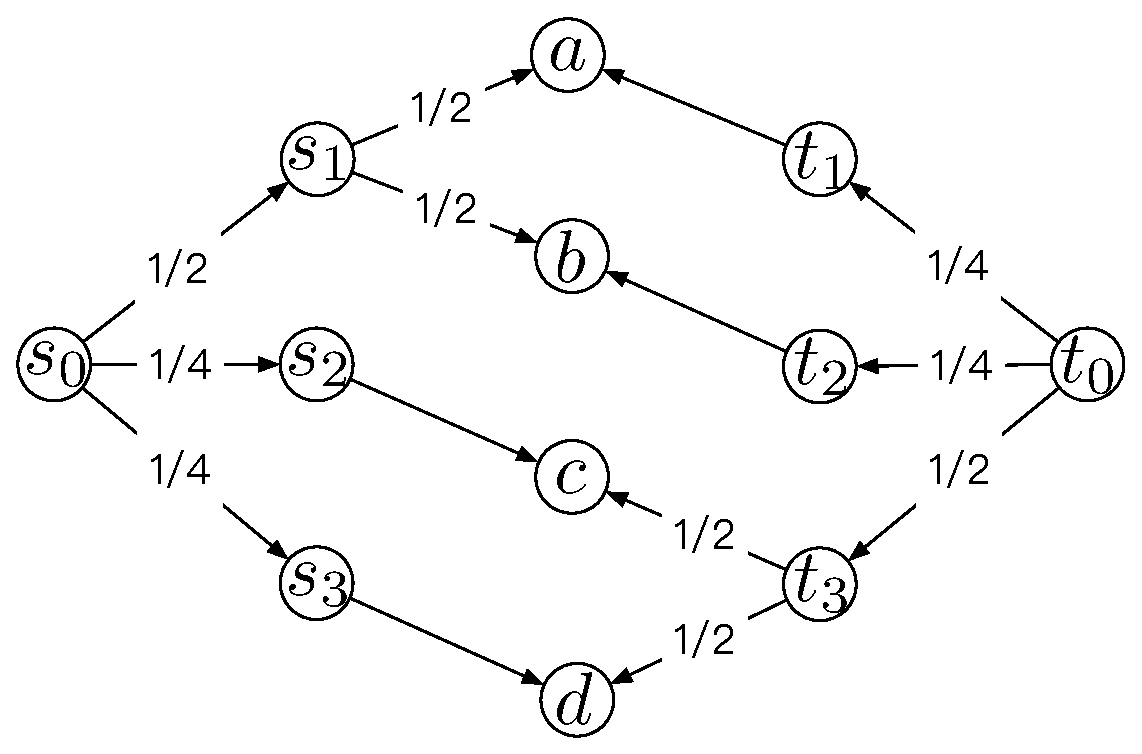
\includegraphics[width=0.5\textwidth]{images/ex.eps}
    \caption{The example.}
    \label{fig:example}
\end{figure}

\section{The Algorithm}
\label{sec:distribution-based bisimulation algorithm}
In this section, we introduce an algorithm to check the distribution-based bisimulation between two pLTSs with fixed initial quantum configurations. We use the algorithm in~\cite{HKK14} to check the distribution-based bisimulation between such pLTSs. The algorithm try finding a characteristic matrix of the equivalence relation.

\begin{definition}\label{def:chara_matrix}
A matrix $E$ is a characteristic matrix of a relation $\mathcal{R}$ if for any $\mu,\nu\in\mathbb{R}^{n}$,
\[\mu\aRel\nu~~~\textbf{iff}~~~(\mu-\nu)E=0.\]
\end{definition}

The relation between the characteristic matrix and the equivalence relation. There are several properties for the relations need to declare first. 

Let $\mathbb{P}^{n}\subseteq\mathbb{R}^{n}$ be the set of probability vectors.
\begin{definition}\label{def:continuous_relation}
A relation $\aRel$ on $\mathbb{P}^{n}$ is said to be continuous if 
\[\mu_{i}\aRel\nu_{i}\wedge\lim_{i\rightarrow\infty}\mu_{i}=\mu\wedge\lim_{i\rightarrow\infty}\nu_{i}=\nu\implies\mu\aRel\nu.\]
\end{definition}

\begin{lemma}\label{lem:affine_relation}
If the relation $\aRel$ is a convex and continuous equivalence relation over probability distributions then $\aRel$ is affine as well. That is for any $\mu_{i}\aRel\nu$ where $i\in\{1,2\}$, $\forall p\in\mathbb{R}^{n}$, there is $\mu=p\mu_{1}+(1-p)\mu_{2}$ and $\mu\aRel\nu$ provided that $\mu\in\mathbb{P}^{n}$.
\begin{proof}
We consider the problem in two cases.
If $0\leq p\leq1$, then from the convexity of $\aRel$, we have $ \mu=p\mu_{1}+(1-p)\mu_{2}$ directly.

Otherwise, without loss of generality, suppose $p<0$. Let $p^{*}=\dfrac{-p}{1-p}$, then there is $0\leq p^{*}\leq1$. Note that $\mu_{2}=(1-p^{*})\mu+p^{*}\mu_{1}$. So we have 
\[\mu_{2}\aRel(1-p^{*})\mu+p^{*}\mu_{1}\aRel\nu.\]
From the result of first case, as $\mu_{1}\aRel\nu$ and $\mu_{2}\aRel\nu$, we can swap $\mu_{1}$ with $\mu_{2}$ here.
Then we have
\[\mu_{2}\aRel(1-p^{*})\mu+p^{*}[(1-p^{*})\mu+p^{*}\mu_{1}]\]
\[\mu_{2}\aRel[1-(p^{*})^{n}]\mu+(p^{*})^{n}\mu_{1}\]
for all $n\geq 0$.
Thus $\mu\aRel\mu_2$ when $n$ tends to infinity as $\aRel$ is continuous, and we get $\mu\aRel\nu$.
\end{proof}
\end{lemma}

\begin{lemma}\label{lem:relation_matrix}
A relation $\aRel$ is a convex and continuous equivalence relation over $\mathbb{P}^{n}$ if and only if there is a characteristic matrix $E$ of it.
\begin{proof}
If there is a characteristic matrix $E$ of $\aRel$. It is obvious that $\aRel$ is a convex and continuous equivalence relation.

For the necessity part, suppose $\mathcal{R}$ is a convex equivalence relation and define the set $\Gamma$ as follow
\[\Gamma = \{\mu-\nu|\mu\aRel\nu, \mu,\nu\in\mathbb{P}^{n}\}.\]
Then let $\overline{\Gamma}$ be the affine closure of $\Gamma$, for any $\rho_{i}\in\Gamma$ and $p_{i}\in\mathbb{R}\wedge \sum_{i}p_{i}=1$, there is $\sum_{i}p_{i}\rho_{i}\in\overline{\Gamma}$. As $\aRel$ is a reflexive relation, there is $\mu-\mu=\textbf{0}\in\Gamma$, and there also exists $\textbf{0}\in\overline{\Gamma}$. For any $\rho'\in\overline{\Gamma}$ and $\rho_{i}\in\overline{\Gamma}$,  $p_{i}\in\mathbb{R}\wedge\sum_{i}p_{i}\neq1$, we can take $p'=1-\sum_{i}p_{i}$ and $p'+\sum_{i}p_{i}=1$, such that
\[p'\rho' + \sum_{i}p_{i}\rho_{i}\in\overline{\Gamma}.\]

Let $\rho'=\textbf{0}$, then we have $\sum_{i}p_{i}\rho_{i}\in\overline{\Gamma}$ for some $\rho_{i}\in\Gamma$. So for any $p_{i}\in\mathbb{R}$, there is $\sum_{i}p_{i}\rho_{i}\in\overline{\Gamma}$ for some $\rho_{i}\in\overline{\Gamma}$. Hence $\overline{\Gamma}$ is a linear subspace of $\mathbb{R}^{n}$.

Therefore, there exists a matrix $E$ whose columns consist of an orthonormal basis of the kernal space of $\overline{\Gamma}$ such that for any $\rho\in\mathbb{R}^{n}$,
\[\rho\in\overline{\Gamma}~~~\textbf{iff}~~~\rho E=0.\]

We are going to show that $E$ is a characteristic matrix for $\aRel$. For any $\mu,\nu\in\mathbb{P}^{n}$, if $\mu~\mathcal{R}~\nu$, let $\rho=\mu-\nu$, $\rho\in\Gamma$, then from $\Gamma\subseteq\overline{\Gamma}$ we have $\rho\in\overline{\Gamma}$ thus $\rho E=0$.

Conversely, suppose $(\mu-\nu)E=0$, then $(\mu-\nu)\in\overline{\Gamma}$. There is a collection of $\{\mu_{i}\}$ and $\{\nu_{i}\}$ s.t. $\mu-\nu=\sum_{i}p_{i}(\mu_{i}-\nu_{i})$ and $\forall i, \mu_{i}\aRel\nu_{i}$. Note that 
\[\mu=\sum_{i}p_{i}\mu_{i}-\sum_{i}p_{i}\nu_{i}+\nu\]
\[\nu=\sum_{i}p_{i}\mu_{i}-\sum_{i}p_{i}\mu_{i}+\nu.\]
Thus according to Lemma~\ref{lem:affine_relation}, $\aRel$ is affine, so we have $\mu\aRel\nu$. 
From Definition~\ref{def:chara_matrix}, $E$ is a characteristic matrix of $\mathcal{R}$ .
\end{proof}
\end{lemma}

% \begin{lemma}\label{lem:relation_matrix}
% A relation $\aRel$ is a convex equivalence relation over possibility distributions if and only if there is a characteristic matrix $E$ of it.
% \begin{proof}
% Let $\aRel$ be any relation on $\mathbb{R}^{n}$ and $\mu, \nu$ be any possibility distribution. So $\mu$ and $\nu$ are also vectors on $\mathbb{R}^{n}$.

% If there is a characteristic matrix $E$ of $\aRel$. For any $\mu,\nu\in Dist(S),\mu\aRel\nu$, there is $(\mu-\nu)E=0$. Then we have $(\nu-\mu)E=0$ which implies $(\nu-\mu)\in\Gamma$ and $\nu\aRel\mu$. So $\aRel$ is a symmetric relation.

% For any $\mu,\nu,\omega\in Dist(S),\mu\aRel\nu,\nu\aRel\omega$, there is $(\mu-\nu)E=0$ and $(\nu-\omega)E=0$. Then we have $(\mu-\omega)E=0$ which implies $(\mu-\omega)\in\Gamma$ and $\mu\aRel\omega$. So $\aRel$ is a transitive relation.

% As $\mu\aRel\nu$ and $\nu\aRel\mu$ exist, and $\aRel$ is a transitive relation, there is $\mu\aRel\mu$. So $\aRel$ is a reflexive relation.

% For each $i\in I,\mu_{i},\nu_{i}\in Dist(S),\mu_{i}\aRel\nu_{i}$, there is $(\mu_{i}-\nu_{i})E=0$. Then for any set of $p_{i}\in\mathbb{R}$ where $p_{i}>0\wedge\sum_{i}p_{i}=1$, there is $p_{i}(\mu_{i}-\nu_{i})=0$. Then their sum $\sum_{i}p_{i}(\mu_{i}-\nu_{i})=0$ implies that $\sum_{i}p_{i}\mu_{i}\aRel\sum_{i}p_{i}\nu_{i}$. So $\aRel$ is a convex relation. As a reuslt, $\aRel$ is a convex equivalence relation.

% In the other direction, suppose $\mathcal{R}$ is a convex equivalence relation and define the set $\Gamma$ as follow
% \[\Gamma = \{\mu-\nu|\mu\aRel\nu\text{ and $\mu,\nu$ are possibility distributions so that }\mu,\nu\in\mathbb{R}^{n}\}.\]
% % Then we prove that
% % \begin{itemize}
% %     \item Claim 1: $\Gamma$ is a vector subspace;
% %     \item Claim 2: $\Gamma$ is independent of $\mu,\nu$.
% % \end{itemize}
% % As to Claim 1, we need to show that $\Gamma$ is closed under $vector$ $addition$ and $scalar$ $multiplication$.

% For any $\rho_{i}\in\Gamma$, let $\rho_{i}=\mu_{i}-\nu_{i}$ where  $\mu_{i}\aRel\nu_i$. 
% By the convexity of $\mathcal{R}$, for any $p_{i}\in\mathbb{R}\wedge p_{i}\geq 0\wedge \sum_{i}p_{i}=1$, \[\sum_{i}p_{i}\mu_{i}\aRel\sum_{i}p_{i}\nu_{i}\implies\sum_{i}p_{i}\mu_{i}-\sum_{i}p_{i}\nu_{i}\in\Gamma\implies\sum_{i}p_{i}(\mu_{i}-\nu_{i})=\sum_{i}p_{i}\rho_{i}\in\Gamma.\]

% So the set $\Gamma$ is closed under convex combinations. Then let $\overline{\Gamma}$ be the affine closure of $\Gamma$, for any $\rho_{i}\in\Gamma$ and $p_{i}\in\mathbb{R}\wedge \sum_{i}p_{i}=1$, there is $\sum_{i}p_{i}\rho_{i}\in\overline{\Gamma}$. The set $\overline{\Gamma}$ is closed under affine combinations and $\Gamma\subseteq\overline{\Gamma}$.

% % Then as $\aRel$ is a symmetric relation, for some $\mu_{j}\aRel\nu_{j}$ and $(\mu_{j}-\nu_{j})\in\Gamma$, there is $\nu_{j}\aRel\mu_{j}$ and $(\nu_{j}-\mu_{j})\in\Gamma$, so we have $p_{j}\geq 0$ and $p_{k}=-p_{j}\leq 0$ such that
% % \[\sum_{i}p_{i}(\mu_{i}-\nu_{i})+p_{j}(\mu_{j}-\nu_{j})+p_{k}(\mu_{j}-\nu_{j})\in\Gamma.\]

% As $\aRel$ is a reflexive relation, there is $\mu-\mu=\textbf{0}\in\Gamma$, and there also exists $\textbf{0}\in\overline{\Gamma}$.

% For any $\rho'\in\overline{\Gamma}$ and $\rho_{i}\in\overline{\Gamma}$,  $p_{i}\in\mathbb{R}\wedge\sum_{i}p_{i}\neq1$, we can take $p'=1-\sum_{i}p_{i}$ and $p'+\sum_{i}p_{i}=1$, such that
% \[p'\rho' + \sum_{i}p_{i}\rho_{i}\in\overline{\Gamma}.\]

% Let $\rho'=\textbf{0}$, then we have $\sum_{i}p_{i}\rho_{i}\in\overline{\Gamma}$ for some $\rho_{i}\in\Gamma$. So for any $p_{i}\in\mathbb{R}$, there is $\sum_{i}p_{i}\rho_{i}\in\overline{\Gamma}$ for some $\rho_{i}\in\overline{\Gamma}$. Hence $\overline{\Gamma}$ is a linear subspace.

% For any $\mu,\nu,\mu',\nu'\in Dist(S)$, let $\Gamma=\{\mu-\nu|\mu~\mathcal{R}~\nu\}, \Gamma'=\{\mu'-\nu'|\mu'~\mathcal{R}~\nu'\}$. Then there is $\Gamma=\Gamma'$. So $\Gamma$ is independent of $\mu,\nu$. Furthermore, as any $\rho\in\overline{\Gamma}$ is the affine combination of elements in $\Gamma$, $\overline{\Gamma}$ is independent of $\mu,\nu$.

% Since $\overline{\Gamma}$ is a linear subspace and it is independent of the choice of $\mu,\nu$, there exists a matrix $E$ such that $\rho\in\overline{\Gamma}$ iff $\rho E=0$. Moreover, for any possibility distributions $\mu,\nu$, $\mu~\mathcal{R}~\nu$, let $\rho=\mu-\nu$, if $\rho\in\Gamma$ then from $\Gamma\subseteq\overline{\Gamma}$ we have $\rho\in\overline{\Gamma}$ and $\rho E=0$.

% And then if $\rho=\mu-\nu$ and $\rho E=0$, we have $\rho\in\overline{\Gamma}$. Furthermore, if $\mu,\nu$ are both possibility distributions, we have $\rho\in\Gamma$ and thus $\mu~\mathcal{R}~\nu$.

% From Definition~\ref{def:chara_matrix}, $E$ is a characteristic matrix of $\mathcal{R}$ .
% \end{proof}
% \end{lemma}

Then we apply the lemmas to the quantum configuration distributions. In order to represent $\sim$ using linear algebra, we index all the configurations in the pLTSs so that every distribution of configurations has its corresponding distribution of indexes which is in a space of real value. Given a set of configurations $S$, if we give a linear order on the state space $S=\{s_1,s_2,\dots,s_n\}$, we can see that the spaces $\mathbb{R}^{n}$ and $\mathbb{R}^{|S|}$ are isomorphic, so do the spaces $\mathbb{P}^{n}$ and $\mathbb{P}^{|S|}$. And obviously, $\mathbb{P}^{|S|}=Dist(S)$. So the distribution $\Delta$ can be presented in form of a real-valued vector $(\Delta(s_1),\cdots,\Delta(s_{|S|}))$.

Then we can find a characteristic matrix $E$ of the distribution-based quantum ground bisimulation as it is also a convex and continuous equivalence relation.

\begin{lemma}\label{lem:bisim_is_rel}
$\sim$ is a convex and continuous equivalence relation.
\begin{proof}
First, according to Definition~\ref{def:dis_strong_bisim}, we have already known that $\sim$ is a equivalence relation. 

Then we prove its convexity. Let $p\in\mathbb{R}$, we show that for any $\Delta_1\sim\Theta_1,\Delta_2\sim\Theta_2$, there is $\Delta\sim\Theta$ where $\Delta=p\Delta_1+(1-p)\Delta_2$ and $\Theta=p\Theta_1+(1-p)\Theta_2$.

We can prove following conditions.
\begin{itemize}
    \item From $qv(\Delta_1)=qv(\Theta_1)$ and $qv(\Delta_2)=qv(\Theta_2)$, we have $qv(\Delta)=qv(\Delta_1)\cup qv(\Delta_2)=qv(\Theta_1)\cup qv(\Theta_2)=qv(\Theta)$.
    \item From $|\Delta_1|=|\Theta_1|$ and $|\Delta_2|=|\Theta_2|$, we have $|\Delta|=|p\Delta_1+(1-p)\Delta_2|=p|\Delta_1|+(1-p)|\Delta_2|=p|\Theta_1|+(1-p)|\Theta_2|=|\Theta|$.
    \item For any $\Delta_1\ar{\alpha}\Delta'_1$, there exists $\Theta'_1$, $\Theta_1\ar{\alpha}\Theta'_1\wedge\Delta'_1\sim\Theta'_1$. So do the $\Delta_2$ and $\Theta_2$. Since $\Delta'=p\Delta'_1+(1-p)\Delta'_2\sim p\Theta'_1+(1-p)\Theta'_2=\Theta'$, for any $\Delta\ar{\alpha}\Delta'$ there is $\Theta'$ such that $\Theta\ar{\alpha}\Theta'\wedge\Delta'\sim\Theta'$.
\end{itemize}
According to Definition~\ref{def:dis_strong_bisim}, it comes out that there is $\Delta\sim\Theta$.

Then we show that it is continuous. That is for any $i\in I$, $\Delta_{i},\Theta_{i}\in Dist(S)$, $\Delta_{i}\sim\Theta_{i}\wedge\lim_{i\rightarrow\infty}{\Delta_{i}}=\Delta\wedge\lim_{i\rightarrow\infty}{\Theta_{i}}=\Theta$ implies that $\Delta\sim\Theta$. For the first  conditions, $\Delta_{i}$ should keep the same set of quantum variables as $\Theta_{i}$. When $\Delta_{i}$ tends to $\Delta$ this set does not changed, so the first condition holds. Similarly, $|\Delta|=|\Theta|$ holds.

For the transition $\Delta_{i}\ar{\alpha}\Delta'_{i}$, there exists transition $\Theta_{i}\ar{\alpha}\Theta'_{i}$ such that $\Delta'_{i}\sim\Theta'_{i}$. When $\Delta_{i}$ tends to $\Delta$, suppose $\Delta'_{i}$ tends to a distribution $\Delta'$. Similarly, a distribution $\Theta'$ is supposed. As $\Delta_{i}$ and $\Theta_{i}$ always keep the relation $\Delta_{i}\sim\Theta_{i}$, we have $\Delta'\sim\Theta'$. Then there is $\Delta\sim\Theta$.
\end{proof}
\end{lemma}

\begin{lemma}\label{lem:matrix_bisim}
There is a characteristic matrix $E$ such that for any $\Delta,\Theta\in Dist(S)$ we have $\Delta\sim\Theta$ iff $(\Delta-\Theta)E=0$.
\begin{proof}
For any distribution $\Delta\in Dist(S)$, there is a vector $\Delta^{o}\in \mathbb{P}^{n}$ s.t. $\Delta(s_{i})=\Delta^{o}(i)$ for each $i$.

For any bisimulation $\mathcal{R}\subseteq Dist(S)\times Dist(S)$, there exists the relation $\mathcal{R}^{o}\subseteq\mathbb{P}^{n}\times\mathbb{P}^{n}$ s.t. $\Delta~\mathcal{R}~\Theta$ iff $\Delta^{o}~\mathcal{R}^{o}~\Theta^{o}$. 

By following Lemma~\ref{lem:bisim_is_rel}, we have $\sim^{o}$ is a convex and continuous equivalence relation. Let $\mathscr{R}$ be the set of all convex and continuous equivalence relations $\mathcal{R'}\subseteq\mathbb{R}^{n}\times\mathbb{R}^{n}$. By Lemma~\ref{lem:relation_matrix}, since $\sim^{o}\in \mathscr{R}$, there is a characteristic matrix $E$ of $\sim^{o}$. As a consequence, for any subdistribution $\Delta,\Theta$, we have
\[\Delta\sim\Theta~~~\textbf{iff}~~~\Delta^{o}\sim^{o}\Theta^{o}~~~\textbf{iff}~~~(\Delta^{o}-\Theta^{o})E=0.\]
\end{proof}
\end{lemma}

We introduce the algorithm in~\cite{HKK14} to find the characteristic matrix $E$ of the quantum bisimulation relation, called the bisimulation matrix, through a transition matrix generated from the configurations of the pLTSs. The transition matrix shows the change of the distributions of states.

% Similarly, we can construct a matrix of superoperators applying on the density operator through each transition between two configuration. Furthermore, if there is non-deterministic choice in the pLTS, there will exist variables in the transition matrix.

\subsection{Action-deterministic Systems}
We first consider checking bisimulation between action-deterministic pLTSs.

Let $P_{\alpha}=(\mathcal{E}_{ij})$ denote the superoperator matrix for each action $\alpha\in\textbf{Act}_{\tau}$ such that for all $i,j$, if there is $\pair{t_{i}, \rho_i}\xrightarrow{\alpha}\Delta$ and $\Delta=\sum_{j}p_{ij}\pair{t_{j}, \mathcal{E}(\rho_{i})}$, $\mathcal{E}_{ij}$ is set to the superoperator $\mathcal{E}$, otherwise it is set to the zero operator $O$.

Furthermore, given an input quantum state we can compute the possibility $p_{ij}$ and construct a real-valued transition matrix. Let $P_{\alpha}(\rho)=(p_{ij})$ denote the transition matrix for each action $\alpha\in\textbf{Act}_{\tau}$ and input quantum state $\rho\in D(\mathcal{H})$ where $D(\mathcal{H})$ is the set of the density operators. 
% For all $i,j$, if $s_{i}=\langle t_{i},\rho_{i}\rangle$, then $p_{ij}$ is set to $\Delta(s_{j})$ which equals to $tr(\mathcal{E}_{ij}(\rho_{i}))$, otherwise it is set to $0$.

We denote $\textbf{1}=(1,\cdots,1)^{\top}$. 
The stability of the matrix $E$ is required to present the second condition of Definition~\ref{def:dis_strong_bisim} which means that for any pair of distributions, if they are contained in $\aRel$, their next distributions are also contained.

\begin{definition}\label{def:p_stable}
For a matrix $E$ with $|S|$ rows and a $|S|\times|S|$ matrix $P$, $E$ is said $P\text{-}stable$ if for every distribution $\Delta$,
\[\Delta E = 0\longrightarrow\Delta P E = 0.\]
\end{definition}

Let matrix $P$ to be the transition matrix of the pLTS, then the distribution $\Delta P$ is the result distribution after one step of movement and it should be still contained in the bisimulation relation. 

\begin{proposition}
\label{prop:bisimulation_deterministic_qlts}
Between two pLTSs $\langle S_1,\textbf{Act}_{\tau},\rightarrow_1 \rangle$ and $\langle S_2,\textbf{Act}_{\tau},\rightarrow_2 \rangle$ with no non-deterministic choice, a $(|S_1|+|S_2|)$ rows real-valued matrix $E$ containing $\textbf{1}$ is a bisimulation matrix if and only if it is $P_{\alpha}(\rho)\text{-}stable$ for all $\alpha\in\textbf{Act}_{\tau}$. For those states whose corresponding positions are non-zero in the same column, their sets of quantum variables should also be the same.
\begin{proof}
Let $\Delta,\Theta\in Dist(S)$ be the distributions from two pLTSs and $\Delta\aRel\Theta$. If $E$ containing $\textbf{1}$ is a bisimulation matrix, there is $(\Delta-\Theta)E=0$ by Lemma~\ref{lem:relation_matrix}. Since $E$ containing $\textbf{1}$, we have $|\Delta|=|\Theta|$. Let $\Delta'=\Delta P_{\alpha}$, then $\Delta\ar{\alpha}\Delta'$. According to definition, there exists $\Theta'=\Theta P_{\alpha}$, $\Theta\ar{\alpha}\Theta'\wedge\Delta'\aRel\Theta'$. Therefore, $(\Delta'-\Theta')E=(\Delta P_{\alpha}-\Theta P_{\alpha})E=(\Delta-\Theta)P_{\alpha}E=0$.
Conversely, let $E$ be a matrix containing $\textbf{1}$ and $P_{\alpha}(\rho)\text{-}stable$ for all $\alpha\in\textbf{Act}_{\tau}$. We show that $\aRel$ defined by $\Delta\aRel\Theta$ iff $(\Delta-\Theta)P_{\alpha}E=0$ for $\Delta,\Theta\in Dist(S)$ is a bisimulation relation. According to Definition~\ref{def:dis_strong_bisim}, as the non-zero value in the same column present the states could be matched, the set of the quantum variables of the distributions to match are the same. So $qv(\Delta)=qv(\Theta)$. Then $\sum_{i}p_{i}tr_{qv(\Delta)(\rho_{i})}=\sum_{j}q_{j}tr_{qv(\Theta)(\sigma_{j})}$ follows from $(\Delta-\Theta)P_{\alpha}\textbf{1}=0$. As $E$ is $P_{\alpha}(\rho)\text{-}stable$, the second condition follows from $(\Delta P_{\alpha}-\Theta P_{\alpha})E=0$. Thus $\aRel$ is a bisimulation relation.
\end{proof}
\end{proposition}

Given $\rho\in D(\mathcal{H})$, the set of all column of $E$ is given by the iteration $\{P_{\alpha}(\rho):\alpha\in\textbf{Act}_{\tau}\}^*\textbf{1}$ modulo linear dependency. Since $P_{\alpha}$ has $|S_1|+|S_2|$ rows, the fixed point reached within $|S_1|+|S_2|$ iterations yielding $1\leq d\leq(|S_1|+|S_2|)$ equations.

% \begin{example}
% We illustrate two quantum processes $Q_1$ and $Q_2$, both of them can set a quantum variable $q_1$ of arbitrary initial value into $|0\rangle$. Let
% \begin{align*}
% Q_{1} &\overset{def}{=} M_{0,1}[q_1;x].(\textbf{if } x=0 \textbf{ then } \mathcal{I}[q_1].\textbf{nil} + \textbf{if } x=1 \textbf{ then } \mathcal{X}[q_1].\textbf{nil})\\
% Q_{2} &\overset{def}{=} Set_{0}[q_1].\mathcal{I}[q_1].\textbf{nil}
% \end{align*}
% where $Set_0=\{|0\rangle\langle 0|,|0\rangle\langle 1|\}$, $\mathcal{I}=\{I\}$, $\mathcal{X}=\{X\}$ and $M_{0,1}$ is a measurement according to the computational basis $\{|0\rangle,|1\rangle\}$.
% Starting at the initial state, as the probability depending on the current quantum state, we can compute the transition matrix 
% \begin{equation*}
% P_{\tau}(\rho)=
% \begin{bmatrix}
% 0 & tr(\mathcal{A}_0\rho) & tr(\mathcal{A}_1\rho) & 0 & 0 & 0 & 0 & 0 \\
% 0 & 0 & 0 & tr(\mathcal{I}\rho_0) & 0 & 0 & 0 & 0 \\
% 0 & 0 & 0 & 0 & tr(\mathcal{X}\rho_1) & 0 & 0 & 0 \\
% 0 & & & \cdots & & & & 0 \\
% 0 & & & \cdots & & & & 0 \\
% 0 & 0 & 0 & 0 & 0 & 0 & tr(Set_{0}\rho) & 0 \\
% 0 & 0 & 0 & 0 & 0 & 0 & 0 & tr(\mathcal{I}Set_{0}\rho) \\
% 0 & & & \cdots & & & & 0 \\
% \end{bmatrix}
% % P_{\tau}=
% % \begin{bmatrix}
% % 0 & \mathcal{A}_0 & \mathcal{A}_1 & 0 & 0 & 0 & 0 & 0 \\
% % 0 & 0 & 0 & \mathcal{I} & 0 & 0 & 0 & 0 \\
% % 0 & 0 & 0 & 0 & \mathcal{X} & 0 & 0 & 0 \\
% % 0 & & & \cdots & & & & 0 \\
% % 0 & & & \cdots & & & & 0 \\
% % 0 & 0 & 0 & 0 & 0 & 0 & Set_{0} & 0 \\
% % 0 & 0 & 0 & 0 & 0 & 0 & 0 & \mathcal{I} \\
% % 0 & & & \cdots & & & & 0 \\
% % \end{bmatrix}
% \end{equation*}
% where $\rho_0 = \dfrac{\mathcal{A}_0\rho}{tr(\mathcal{A}_0\rho)}$ and $\rho_1 = \dfrac{\mathcal{A}_1\rho}{tr(\mathcal{A}_1\rho)}$.

% By two times of iterations, we can get the columns of the bisimulation matrix.

% \begin{equation*}
% P_\tau(\rho)\textbf{1}=\begin{bmatrix}
% tr(\mathcal{A}_0\rho)+tr(\mathcal{A}_1\rho)\\
% tr(\mathcal{I}\rho_0)\\
% tr(\mathcal{X}\rho_1)\\
% 0\\
% 0\\
% tr(Set_{0}\rho)\\
% tr(\mathcal{I}Set_{0}\rho)\\
% 0\\
% \end{bmatrix}=\begin{bmatrix}
% 1\\
% 1\\
% 1\\
% 0\\
% 0\\
% 1\\
% 1\\
% 0\\
% \end{bmatrix}
% \end{equation*}
% \begin{align*}
% P_{\tau}(\rho)P_{\tau}(\rho)\textbf{1}&=\begin{bmatrix}
% tr(\mathcal{A}_0\rho)tr(\mathcal{I}\rho_0)+tr(\mathcal{X}\mathcal{A}_1\rho)tr(\mathcal{X}\rho_1)\\
% 0\\
% 0\\
% 0\\
% 0\\
% tr(Set_{0}\rho)tr(\mathcal{I}Set_{0}\rho)\\
% 0\\
% 0\\
% \end{bmatrix}=
% % \begin{bmatrix}
% % tr(\mathcal{I}\mathcal{A}_0\rho)+tr(\mathcal{X}\mathcal{A}_1\rho)\\
% % 0\\
% % 0\\
% % 0\\
% % 0\\
% % tr(\mathcal{I}Set_{0}\rho)\\
% % 0\\
% % 0\\
% % \end{bmatrix}=
% \begin{bmatrix}
% 1\\
% 0\\
% 0\\
% 0\\
% 0\\
% 1\\
% 0\\
% 0\\
% \end{bmatrix}
% \end{align*}
% where $\rho_0 = \dfrac{\mathcal{A}_0\rho}{tr(\mathcal{A}_0\rho)}$ and $\rho_1 = \dfrac{\mathcal{A}_1\rho}{tr(\mathcal{A}_1\rho)}$.

% Then we have the bisimulation matrix $E = ( \textbf{1}~~P_{\tau}(\rho)\textbf{1}~~P_{\tau}(\rho)P_{\tau}(\rho)\textbf{1} )$. If we want to check the initial distributions $\Delta, \Theta$ of two processes $P_1$ and $P_2$ where 
% \[\Delta = (1,0,\cdots,0)~\text{ and }~\Theta = (0,\cdots,0,1,0,0).\]
% According to Proposition~\ref{prop:bisimulation_deterministic_qlts}, there is $(\Delta-\Theta)E = 0$, so there must exist the equations $tr(\mathcal{A}_0\rho)+tr(\mathcal{A}_1\rho)=tr(Set_{0}\rho)$ and $tr(\mathcal{I}\mathcal{A}_0\rho)+tr(\mathcal{X}\mathcal{A}_1\rho)=tr(\mathcal{I}Set_{0}\rho)$ which are the required conditions of $\Delta\aRel^{D}\Theta$.
% \end{example}

\subsection{Non-deterministic Systems}
Then we consider checking bisimulation between pLTSs containing non-deterministic choices.

When there exists non-deterministic choices in the pLTS, the transition matrix $P_{\alpha}(\rho)$ may contain symbolic variables used to present the probability of a transition will be taken. For each $\pair{t_{i}, \rho_i}\in S$, $\alpha\in \textbf{Act}_{\tau}$, let $c^{\alpha}_{i}$ be the number of non-deterministic choices of $\pair{t_{i}, \rho_i}$ under action $\alpha$, $w^{k}_{i}$, $0\leq k\leq c^{\alpha}_{i}$ be the probability that the $k$-th choice is taken. 

Let the transition be $\pair{t_{i}, \rho_i}\xrightarrow{\alpha}\Delta^{k}_{i}$ where $\Delta^{k}_{i}=\sum_{j}p^{k}_{ij}\pair{t_{j}, \rho_j}$. Let the collection $W$ keeps the probability of each choice and the matrix $P^{W}_{\alpha}(\rho)$ sums up the choices under action $\alpha$. 
Then the transition matrix is presented as $P^{W}_{\alpha}(\rho) = (\sum^{c^{\alpha}_{i}}_{k=1}w^{k}_{i}\cdot p^{k}_{ij})$. 

% Furthermore, we consider the superoperator-valued distribution together with the non-deterministic choice. For any $\rho\in D(\mathcal{H})$, let
% \begin{equation*}
% \rho=
% \begin{bmatrix}
% a_{11} & \cdots & a_{1n} \\
% \vdots & \ddots & \vdots \\
% a_{n1} & \cdots & a_{nn}
% \end{bmatrix}
% \end{equation*}
% where $a_{11},a_{22},\cdots,a_{nn}\geq 0$ and $\sum^{n}_{i=1}a_{ii} = 1$. Then we define $P^{W}_{\gamma}(\rho)$ taking $\rho$ as an input to each element of it and computing their trace. Let $f^{j}_{s}(a_{11},\cdots,a_{ii})=tr(\Delta^{j}_{i}(s)(\rho))$ then the $i$-th row of $P^{W}_{\gamma}(\rho)$ is $\sum^{c^{\gamma}_{i}}_{j=0}w^{j}_{i}tr(\Delta^{j}_{i}(\rho))=\sum^{c^{\gamma}_{i}}_{j=0}w^{j}_{i}[\sum_{s_{k}\in\lceil\Delta^{j}_{i}\rceil}f^{j}_{s_k}(a_{11},\cdots,a_{ii})]$.

The value of the $w^{k}_{i}$ is taken by a Spoiler-Duplicator bisimulation game in $s_{i}$. That is, for a pair of distribution $\{\Delta_{0},\Delta_{1}\}$, Spoiler chooses $i\in\{0,1\}$, $\alpha\in\mathsf{Act}$, $\Delta_{i}\ar{\alpha}\Delta'_{i}$ and Duplicator has to reply 
$\Delta_{1-i}\ar{\alpha}\Delta'_{1-i}$ such that $\Delta_{i}(S_{\alpha})=\Delta_{1-i}(S_{\alpha})$, and the game continues in $\{\Delta'_{0},\Delta'_{1}\}$ where $S_{\alpha}$ is a set of states $\{s|\exists\Theta : s\ar{\alpha}\Theta\}$. Spoiler wins the games if and only if Duplicator cannot reply at some point.

The fundamental idea of the algorithm is that if two distributions are matched on the finitely many ``extremal'' choices, we can check they are bisimilar. When we compute the matrix by the same iteration method, there are variable $w^{k}_{i}$ in the matrix $M^{W}_{\alpha}(\rho)=P^{W}_{\alpha}(\rho)E$ where $E$ is the result of the last iteration.
% Moreover, $M^{W}_{\gamma}(\rho)=P^{W}_{\gamma}(\rho)E$.
The $i$-th row of $M^{W}_{\alpha}(\rho)$ over $W$ is a vector containing variables $w^{k}_{i}$, denoted by $m_{il}(w^{1}_{i},\cdots,w^{c^{\alpha}_{i}}_{i})$. As there are random and mixed choices to take, the set of vectors
\[\{m_{i1}(w^{1}_{i},\cdots,w^{c_{i}}_{i}),\cdots,m_{ib}(w^{1}_{i},\cdots,w^{c_{i}}_{i})|w^{1}_{i},\cdots,w^{c_{i}}_{i}\geq 0,\sum^{c_i}_{k=1}w^{k}_{i}=1\}\]
constructs a convex polytope denoted by $C_{i}$. The extremal points of $C_{i}$ is denoted by $\mathcal{E}(C_i)$. 

For all the rows, $C = \{\sum_{i=1}^{|S|}c'_{i}|\forall i : c'_{i}\in C_{i}\}$ is also a polytope. Let the set $\mathcal{E}(C)\subseteq\prod^{|S|}_{i=1}\mathcal{E}(C_{i})$ contain a tuple $c=(c_{1},\cdots,c_{|S|})$ if and only if they are extremal in the same direction that is $\sum_{i=1}^{|S|}c_{i}$ is a vertex of the polytope. The particular choices corresponding to $c\in \mathcal{E}(C)$ is denoted by $W(c)$. Then the elements of the transition matrix $P^{W(c)}_{\alpha}$ can be confirmed with $W(c)$ plugged in.

Denote the $|S|$-dimensional vector of $C_{i}$'s by $\textbf{C}$. For a distribution $\Delta$, the $\Delta$-combination of polytope $C_{i}$ is
\[\Delta\textbf{C}^{\top}=\{\sum_{i=1}^{|S|}\Delta(s_{i})c_{i}|\forall i : c_{i}\in C_{i}\}.\]
Furthermore, the set $\mathcal{E}(\Delta\textbf{C}^{\top})$ is $\{\Delta c^{\top}|c\in \mathcal{E}(C)\}$. Note that these points are mapped to pure strategies and achieve Pareto extremal values when applied to any distributions, i.e. $\Delta c^{\top}$ is a corner of $\Delta\textbf{C}^{\top}$ for every distribution µ.

\begin{proposition}
\label{prop:bisimulation_nondeterministic_qlts}
Between two pLTSs $\pair{S_1,\textbf{Act}_{\tau},\rightarrow_1}$ and $\pair{S_2,\textbf{Act}_{\tau},\rightarrow_2}$. Let $E$ be a $(|S_1|+|S_2|)$ rows real-valued matrix containing \textbf{1}. It is a bisimulation matrix if and only if it is $P^{W(c)}_{\alpha}(\rho)$-stable for all $\alpha\in L$ and $c\in\mathcal{E}(C)$. For those states whose corresponding positions are non-zero in the same column, their sets of quantum variables should also be the same.
\begin{proof}
Other parts are similar to the proof in Proposition~\ref{prop:bisimulation_deterministic_qlts} except proving $E$ is $P^{W(c)}_{\alpha}(\rho)$-stable for all $\alpha\in L$ and $c\in\mathcal{E}(C)$.

Let $\Delta,\Theta\in Dist(S)$ be the distributions from two pLTSs. Observe that if $\Delta\aRel\Theta$ then $\Delta\textbf{C}^{\top}$ and $\Theta\textbf{C}^{\top}$ are the same polytopes as for every choice on one side there must be a choice on the other side matching it in all states. Conversly, if $\Delta\textbf{C}^{\top}$ and $\Theta\textbf{C}^{\top}$ are not the same, then $\Delta\aRel\Theta$ also does not hold. Spoiler can choose a distribution that cannot be matched by Duplicator. Note that equality of the polytopes $\Delta\textbf{C}^{\top}$ and $\Theta\textbf{C}^{\top}$ can be tested by the equality of the sets of the extremal points $\mathcal{E}(\Delta\textbf{C}^{\top})$ and $\mathcal{E}(\Theta\textbf{C}^{\top})$.
Hence two facts need to be proved:
\begin{itemize}
    \item The extremal choices $\mathcal{E}(C)$ are sufficient for Spoiler, that is $W_{S}=W(c)$.
    \item For an extremal choice $W(c)$ from Spoiler, $W(c)$ is an optimal reply of Duplicator for any distrbutions $\Delta$ and $\Theta$, that is $W_{D}=W(c)$.
\end{itemize}

As to the first fact, intuitively, if two polytopes are different, there must be a corner of one of them not in the other by the convexity of the polytope. If $\Delta\textbf{C}^{\top}$ and $\Theta\textbf{C}^{\top}$ are not the same, then the optimal choice of Spoiler is a $W(c)$ such that $\Delta c^{\top}\not\in\Theta\textbf{C}^{\top}$ (or $\Theta c^{\top}\not\in\Delta\textbf{C}^{\top}$).

As to the second fact, intuitively, if two polytopes are the same and Spoiler checks whether a corner $c_{1}$ is also a corner of the other one, then Duplicator needs to reply the corner $c_{2}$ which is extremal in the same direction as $c_{1}$. Let $\Delta\aRel\Theta$ and $W(s)$ be an extremal choice of Spoiler on $\Delta$, $W(d)$ be an optimal choice of Duplicator on $\Theta$. For a contradiction, suppose $W(d)$ is different from $W(s)$. Since $s$ is extreme in some direction $v$ for which $d$ is not, and since $W(s)$ achieves on $\Delta$ the same as $W(d)$ on $\Theta$, there is a choice $W(d')$ where $d'$ is extreme in direction $v$ and achieves strictly better Pareto value on $\Theta$ than $d$, hence also strictly better than $W(s)$ on $\Delta$. Then if Spoiler choose $W(d)$ on $\Theta$, a matching reply would be $W(s)$ on $\Delta$. Furthermore, if Spoiler choose $W(d')$ on $\Theta$, this choice is strictly dominates $W(d)$ on $\Theta$ in direction $v$ and thus all choices on $\Delta$ in direction $v$, as $s$ is already the extremal choice in direction $v$. Hence Duplicator has no choice to reply, this is a contradiction.

As a result, the bisimulation matrix requirement can be simplified. In the game fashion it is written as follows:
\[\forall\alpha\in\mathsf{Act}, (\Delta-\Theta)E=0\implies\forall W_{S},\exists W_{D},\Delta P^{W_{S}}_{\alpha}\textbf{1}=\Theta P^{W_{D}}_{\alpha}\textbf{1}\wedge(P^{W_{S}}_{\alpha}-\Theta P^{W_{D}}_{\alpha})E=0.\]
Since $W_{S}=W(c)$, $W_{D}=W(c)$ and $E$ contains $\textbf{1}$, there is
\[\forall\alpha\in\mathsf{Act}, (\Delta-\Theta)E=0\implies\forall W(c), (\Delta-\Theta) P^{W(c)}_{\alpha}E=0\]
which shows that $E$ is $P^{W(c)}_{\alpha}(\rho)$-stable for all $\alpha\in L$ and $c\in\mathcal{E}(C)$.
\end{proof}
\end{proposition}

Algorithm~\ref{alg:bisim} computes the bisimulation matrix of a pLTS which may contain non-deterministic choices. The algorithm is divided into two parts.The first part traverses the pLTSs to compute the transition matrix with the input quantum state $\rho\in D(\mathcal{H})$. Then the algorithm compute the columns of $E$ by the iteration $\{P^{W(c)}_{\alpha}:\alpha\in\textbf{Act}_{\tau},W\in\mathcal{W}_{\tau}\}^*\textbf{1}$. According to the condition given in Definition~\ref{def:dis_strong_bisim}, the algorithm also matches the quantum variables of two corresponding distributions when a new column is added (Line 12).

% \begin{example}
% We illustrate two quantum processes $R_1$ and $R_2$. Let
% \begin{align*}
% R_{1} &\overset{def}{=} Q_{1}+Q_{2}\\
% R_{2} &\overset{def}{=} Q_{2}.
% \end{align*}
% We can compute the transition matrix: 
% \begin{equation*}
% P^{W}_{1\tau}(\rho)=
% \begin{bmatrix}
% 0 & w_{1}^{1}tr(\mathcal{A}_0\rho) & w_{1}^{1}tr(\mathcal{A}_1\rho) & w_{1}^{2}tr(Set_{0}\rho) & 0 & 0 & 0\\
% 0 & 0 & 0 & 0 & tr(\mathcal{I}\rho_0) & 0 & 0 \\
% 0 & 0 & 0 & 0  & 0 & tr(\mathcal{X}\rho_1) & 0 \\
% 0 & 0 & 0 & 0  & 0 & 0 & tr(\mathcal{I}Set_{0}\rho) \\
% 0 & & & \cdots & & & 0 \\
% \vdots & & & & & & \vdots \\
% 0 & & & \cdots & & & 0 \\
% \end{bmatrix}
% \end{equation*}
% where $\rho_0 = \dfrac{\mathcal{A}_0\rho}{tr(\mathcal{A}_0\rho)}$ and $\rho_1 = \dfrac{\mathcal{A}_1\rho}{tr(\mathcal{A}_1\rho)}$.

% \begin{equation*}
% P^{W}_{2\tau}(\rho)=
% \begin{bmatrix}
% 0 & tr(Set_{0}\rho) & 0 \\
% 0 & 0 & tr(\mathcal{I}Set_{0}\rho) \\
% 0 & 0 & 0 \\
% \end{bmatrix}.
% \end{equation*}

% The transition matrix $P^{W}_{\tau}(\rho)$ is
% \begin{equation*}
% P^{W}_{\tau}(\rho)=
% \begin{bmatrix}
% P^{W}_{1\tau} & 0 \\
% 0 & P^{W}_{2\tau} \\
% \end{bmatrix}.
% \end{equation*}

% Then after two times of iterations $\{P^{W}_{\tau}(\rho)|\alpha\in\textbf{Act}_{\tau},W\in\mathcal{W}_{\tau}\}^*\textbf{1}$, there is

% \begin{equation*}
% % E = \textbf{1}\ P^{W}_{d!0}(\rho)\textbf{1}\ P^{W}_{d!1}(\rho)\textbf{1}=
% % \begin{bmatrix}
% % 1 & 0 & 0 \\
% % 1 & 1 & 0 \\
% % 1 & 0 & 1 \\
% % \vdots & \vdots & \vdots \\
% % 1 & 0 & 0 \\
% % 1 & 1 & 0 \\
% % 1 & 0 & 1 \\
% % \vdots & \vdots & \vdots \\
% % 1 & 0 & 0 \\
% % \end{bmatrix}
% M^{W}_{\tau}(\rho) = P^{W}_{\tau}(\rho)P^{W}_{\tau}(\rho)\textbf{1}=
% \begin{bmatrix}
% w_{1}^{1}[tr(\mathcal{I}\mathcal{A}_0\rho)+tr(\mathcal{X}\mathcal{A}_1\rho)]+w_{1}^{2}tr(\mathcal{I}Set_{0}\rho)\\
% 0\\
% \vdots\\
% 0\\
% tr(\mathcal{I}Set_{0}\rho)\\
% 0\\
% 0\\
% \end{bmatrix}.
% \end{equation*}
% % \begin{equation*}
% % M^{W}_{\tau}(\rho)=
% % \begin{bmatrix}
% % tr(\mathcal{A}_0(\rho)+\mathcal{A}_1(\rho)) & tr(\mathcal{A}_0(\rho)) & tr(\mathcal{A}_1(\rho)) \\
% % 0 & 0 & 0 \\
% % \vdots & \vdots & \vdots \\
% % 0 & tr(Set) & 0 \\
% % w^{1}_{6}+w^{2}_{6} & w^{1}_{6} & w^{2}_{6} \\
% % 0 & 0 & 0 \\
% % \vdots & \vdots & \vdots \\
% % 0 & 0 & 0 \\
% % \end{bmatrix}=
% % \begin{bmatrix}
% % a_{11}+a_{22} & a_{11} & a_{22} \\
% % 0 & 0 & 0 \\
% % \vdots & \vdots & \vdots \\
% % 0 & tr(Set_{0}\rho) & 0 \\
% % 0 & 0 & tr(\rho) \\
% % 0 & 0 & 0 \\
% % \end{bmatrix}.
% % \end{equation*}
% So there is $C = ((w_{1}^{1},w_{2}^{1}))$. We can take $((1,0))\in\mathcal{E}(C)$ as the ``extremal'' choice, then we get $M^{W(c)}_{\tau}(\rho)=(1,0,\cdots,0,1,0,0)^{\top}$.
% In the other case, we choose $((0,1))\in\mathcal{E}(C)$ and the result is similar. As $E_{new}$ is each column of $M^{W(c)}_{\tau}(\rho(c))$, we have $E = (\textbf{1}~~P^{W(c)}_{\tau}(\rho)\textbf{1}~~M^{W(c)}_{\tau}(\rho))$.
% \end{example}
% Let $\Delta$ and $\Theta$ be the initial configuration of $R_1$ and $R_2$, $(\Delta-\Theta)=(1,\cdots,0,-1,0,0)$. From $(\Delta-\Theta)E=\textbf{0}$, we have equations  $tr(\mathcal{I}\mathcal{A}_0\rho)+tr(\mathcal{X}\mathcal{A}_1\rho)=tr(\mathcal{I}Set_{0}\rho)$ and $tr(\mathcal{I}Set_{0}\rho)=tr(\mathcal{I}Set_{0}\rho)$ , the required condition of $\Delta\aRel^{D}\Theta$.

% Furthermore, if there are $R_1\xrightarrow{\tau}\Delta$, $R_2\xrightarrow{\tau}\Theta$, then $\Delta-\Theta=(0,\mathcal{A}_0,\mathcal{A}_1,0,0,0,-p_0\mathcal{I},-p_1\mathcal{I},0,0)$, $(\Delta-\Theta)E=\textbf{0}$ implies that $\mathcal{A}_0+\mathcal{A}_1~\overline{\sim}~(p_0+p_1)\mathcal{I}$, $\mathcal{A}_0~\overline{\sim}~p_0\mathcal{I}$ and $\mathcal{A}_1~\overline{\sim}~p_1\mathcal{I}$. For any $\rho$, $tr(\mathcal{A}_i(\rho))=p_i tr(\mathcal{I}(\rho))=p_i$ and from $\sum_{i}\mathcal{A}_i~\overline{\sim}~\mathcal{I}$ we have $\sum_{i}p_i=1$, so the conditions are satisfied if we take $p_i = tr(\mathcal{A}_i(\rho))$.


\begin{algorithm}[htbp]
\caption{Checking Symbolic Ground Bisimulation}
\label{alg:bisim}
\begin{algorithmic}[1]
\Require Two pLTSs.
\Ensure A minimal bisimulation matrix $E$.
\Function{\textbf{SymbolicBisimulation}}{} = 
\For{\textbf{each} $\alpha\in L$}
\State traverse the pLTSs to compute $P^{W}_{\alpha}(\rho)$
\EndFor
\State $E\leftarrow(\textbf{1})$
\Repeat
\For{\textbf{each} $\alpha\in L$}
\State $M^{W}_{\alpha}(\rho)\leftarrow P^{W}_{\alpha}(\rho)E$
\State compute $\mathcal{E}(C)$ from $M^{W}_{\alpha}$
\For{\textbf{each} $c\in\mathcal{E}(C)$}
\State $M^{W(c)}_{\alpha}(\rho)\leftarrow M^{W}_{\alpha}(\rho)$ with $W(c)$ plugged in
\For{\textbf{each} column $E_{new}$ in $M^{W(c)}_{\alpha}(\rho)$ independent of $E$}
\State check the sets of quantum variables of non-zero rows
\If{these sets are equal}
\State $E\leftarrow(E ~~ E_{new})$
\Else \textbf{ skip }
\EndIf
\EndFor
\EndFor
\EndFor
\Until{$E$ does not change}
\State \textbf{return} $E$
\EndFunction
\end{algorithmic}
\end{algorithm}

\section{Weak Distribution-based Bisimulation}
\label{sec:weak}
To abstract the invisible actions caused by internal communications, as well as quantum operations, we refer to the idea of saturation which extends an automaton to a weak automaton through adding weak transitions.

We write $\Delta \ar{\hat{\tau}} \Theta$ if either $\Delta \ar{\tau} \Theta$ or $\Theta = \Delta$.
We define weak transitions $\dar{\hat{a}}$ by letting $\dar{\hat{\tau}}$ be the reflexive and transitive closure of $\ar{\hat{\tau}}$ and writing $\Delta\dar{\hat{a}} \Theta$ for $a \in\Act$ whenever $\Delta \dar{\hat{\tau}} \ar{a} \dar{\hat{\tau}} \Theta$.

We denote $P'$ as the pLTS $P$ adding weak transitions according to the following rules.

\begin{figure}[H]
    \centering
    $\begin{array}{lrllrllr}
        weak1 &  \inferrule
            {  }
            {\Delta\xLongrightarrow{\epsilon}\Delta}
        && weak2 &  \inferrule
            {\Delta\xlongrightarrow{\gamma}\Delta}
            {\Delta\xLongrightarrow{\gamma}\Delta}
        % && weak3 &  \inferrule
        %     {\Delta\xlongrightarrow{\tau}\Delta}
        %     {\Delta\xLongrightarrow{\tau}\Delta}
    \end{array}$
    \smallskip
    
    $\begin{array}{lr}
      weak3 &  \inferrule
            {\Delta\xLongrightarrow{\gamma}\sum\nolimits_{s\in\lceil\Delta\rceil}\Delta_{s}\quad\quad\forall s\in\lceil\Delta\rceil:~\Delta_{s}\xlongrightarrow{\tau}\Theta_{s}}
            {\Delta\xLongrightarrow{\gamma}\sum\nolimits_{s\in\lceil\Delta\rceil}\Theta_{s}}
    \end{array}$
    \smallskip
    
    $\begin{array}{lr}
      weak4 & \inferrule
            {\Delta\xlongrightarrow{\tau}\sum\nolimits_{s\in\lceil\Delta\rceil}\Delta_{s}\quad\quad\forall s\in\lceil\Delta\rceil:~\Delta_{s}\xLongrightarrow{\gamma}\Theta_{s}}
            {\Delta\xLongrightarrow{\gamma}\sum\nolimits_{s\in\lceil\Delta\rceil}\Theta_{s}}
    \end{array}$
    \caption{Weak Transition Rules}
    \label{fig:weak_trans}
\end{figure}

Then we can apply the same algorithm in~\ref{sec:distribution-based bisimulation algorithm} to the result pLTSs to check the weak bisimulation.

\section{Experimental Results}
\label{sec:weak_experiment}
We implement the algorithm in Python and then we conducted experiments on several quantum communication protocols with a set of given input variables (both quantum and classical). Firstly, we make a brief introduction about the examples we used.

\noindent\textbf{Measurement on two qubits.} In quantum mechanics, measuring a two-qubit state should be equal to measuring each qubit separately with the same basis. These two ways of measurement can be defined as follows:
\begin{flalign*}
S1 \overset{def}{=}& Set_{\Psi}[q1,q2].M_1[q_1;x_1].(\textbf{if}\ x_1=0\ \textbf{then}\ M_1[q_2;x_2].(\textbf{if}\ x_2=0\ \textbf{then}\ d!0.\textbf{nil} \\
& \qquad\qquad\qquad\qquad\qquad\qquad\qquad\qquad\qquad\qquad\qquad+\textbf{if}\ x_2=1\ \textbf{then}\ d!1.\textbf{nil})\\
& \qquad\qquad\qquad\qquad\quad + \textbf{if}\ x_1=1\ \textbf{then}\ M_1[q_2;x_2].(\textbf{if}\ x_2=0\ \textbf{then}\ d!2.\textbf{nil} \\
& \qquad\qquad\qquad\qquad\qquad\qquad\qquad\qquad\qquad\qquad\qquad+\textbf{if}\ x_2=1\ \textbf{then}\ d!3.\textbf{nil}));\\
S2 \overset{def}{=}& Set_{\Psi}[q1,q2].M_1[q_1, q_2;x_1].(\sum_{i=0}^{3}\textbf{if}\ x_1=i\ \textbf{then}\ d!i.\textbf{nil})
\end{flalign*}
where $Set_{\Psi}[\tilde{q}]$ sets the two-qubit state $|q1\rangle|q2\rangle$ to the state $|+\rangle|+\rangle$.

\noindent\textbf{Communication protocols.} Many quantum protocols use the property of the maximally entangled state, EPR state, to achieve a more efficient communication, such as super-dense coding protocol, teleportation protocol and secret sharing protocol. In these examples, we make the use of their quantum circuit presentation to encode them into qCCS programs and match them with their specifications.

\noindent\textbf{Key distribution protocols.} Quantum key distribution protocols also use the some properties in quantum mechanics to encrypt the key. For example, because of the quantum no-cloning theorem, a third party will be detected if he eavesdrops the qubits. When the protocol randomly decide which key the protocol to transport, it can use the result of a measurement on a qubit which leads to a probability distribution. In another way, non-deterministic choices can be used instead of it to present the randomness of the generation of the key.

Table~\ref{tab:weak_result} provides a summary of our experimental results obtained on a macOS machine with an Intel Core i7 2.5 GHz processor and 16GB of RAM.

In the result of 2-qubit measurement, the distribution-based bisimulation checking algorithm succeed verifying that two processes are bisimilar. From the last column of the table, we can see that with the distribution-based method the bisimulation checking has been finished in less time. The time cost excludes the part of pLTS generation which takes around 1 second in all the examples.

\begin{table}[H]
\footnotesize
\centering
\begin{tabular}{@{}m{0pt}@{}
                >{\centering\arraybackslash}m{3.6cm}
                ||>{\centering\arraybackslash}m{4cm}
                |>{\centering\arraybackslash}m{0.8cm}
                |>{\centering\arraybackslash}m{0.6cm}
                |>{\centering\arraybackslash}m{0.6cm}
                |>{\centering\arraybackslash}m{1cm}}
\hline
\multicolumn{7}{c}{\textbf{State-based weak bisimulation}}\\
\hline
\hline
\rule{0pt}{3mm}&\textbf{Program} & \textbf{Arguments} & \textbf{Bisim} & \textbf{Impl} & \textbf{Spec} & \textbf{Sec} \\
\hline
\hline
\rule{0pt}{3mm} & {\shortstack{Teleportation}} & \tabincell{c}{$q_1q_2q_3=\frac{1}{\sqrt{2}}|000\rangle\text{\tiny{+}}\frac{1}{\sqrt{2}}|100\rangle$} & Yes & 54 & 8 & 1015 \\
\hline
\rule{0pt}{3mm} & {\shortstack{Super-dense coding}} & $q_1q_2=|00\rangle$, $x=5$ & Yes & 8 & 5 & 141 \\
\hline
\rule{0pt}{3mm} & {\shortstack{Secret Sharing}} & \tabincell{c}{$q_1q_2q_3q_4=\frac{1}{\sqrt{2}}|0000\rangle\text{\tiny{+}}\frac{1}{\sqrt{2}}|1000\rangle$} & Yes & 143 & 8 & 5565 \\
\hline
\rule{0pt}{3mm} & BB84 & \tabincell{c}{$q_1q_2q_3=|00\rangle$} & Yes & 152 & 80 & 147792 \\
\hline
\rule{0pt}{3mm} & B92 & \tabincell{c}{$q_1q_2=|00\rangle$} & Yes & 64 & 80 & 32541 \\
\hline
\rule{0pt}{3mm} & E91 & \tabincell{c}{$q_1q_2q_3q_4=|0000\rangle$} & Yes & 124 & 80 & 124015 \\
\hline
\rule{0pt}{3mm} & BB84 (non-deterministic) & \tabincell{c}{$q_1q_2=|00\rangle$} & Yes & 93 & 25 & 21752 \\
\hline
\rule{0pt}{3mm} & B92 (non-deterministic) & \tabincell{c}{$q_1q_2=|00\rangle$} & Yes & 37 & 23 & 2785 \\
\hline
\rule{0pt}{3mm} & E91 (non-deterministic) & \tabincell{c}{$q_1q_2=|00\rangle$} & Yes & 79 & 25 & 1712 \\
\hline
\rule{0pt}{3mm} & 2-qubit measurement & \tabincell{c}{$q_1q_2=|00\rangle$} & No & 12 & 16 & 156 \\
\hline
\hline
\multicolumn{7}{c}{\textbf{Distribution-based weak bisimulation}}\\
\hline
\hline
\rule{0pt}{3mm}&\textbf{Program} & \textbf{Arguments} & \textbf{Bisim} & \textbf{Impl} & \textbf{Spec} & \textbf{Sec} \\
\hline
\hline
\rule{0pt}{3mm} & {\shortstack{Teleportation}} & \tabincell{c}{$q_1q_2q_3=\frac{1}{\sqrt{2}}|000\rangle\text{\tiny{+}}\frac{1}{\sqrt{2}}|100\rangle$} & Yes & 54 & 8 & 252 \\
\hline
\rule{0pt}{3mm} & {\shortstack{Super-dense coding}} & $q_1q_2=|00\rangle$, $x=5$ & Yes & 8 & 5 & 10 \\
\hline
\rule{0pt}{3mm} & {\shortstack{Secret Sharing}} & \tabincell{c}{$q_1q_2q_3q_4=\frac{1}{\sqrt{2}}|0000\rangle\text{\tiny{+}}\frac{1}{\sqrt{2}}|1000\rangle$} & Yes & 143 & 8 & 16143 \\
\hline
\rule{0pt}{3mm} & BB84 & \tabincell{c}{$q_1q_2q_3=|00\rangle$} & Yes & 152 & 80 & 5357 \\
\hline
\rule{0pt}{3mm} & B92 & \tabincell{c}{$q_1q_2=|00\rangle$} & Yes & 64 & 80 & 1390 \\
\hline
\rule{0pt}{3mm} & E91 & \tabincell{c}{$q_1q_2=|0000\rangle$} & Yes & 124 & 80 & 3533 \\
\hline
\rule{0pt}{3mm} & BB84 (non-deterministic) & \tabincell{c}{$q_1q_2=|00\rangle$} & Yes & 93 & 25 & 1177 \\
\hline
\rule{0pt}{3mm} & B92 (non-deterministic) & \tabincell{c}{$q_1q_2=|00\rangle$} & Yes & 37 & 23 & 310 \\
\hline
\rule{0pt}{3mm} & E91 (non-deterministic) & \tabincell{c}{$q_1q_2=|00\rangle$} & Yes & 79 & 25 & 902 \\
\hline
\rule{0pt}{3mm} & 2-qubit measurement & \tabincell{c}{$q_1q_2=|00\rangle$} & Yes & 12 & 16 & 54 \\
\hline
\end{tabular}
\caption{Experimental results. The columns headed by \textbf{Impl} and \textbf{Spec} show the numbers of nodes contained in the generated pLTSs of the implementations and specifications, respectively. Column \textbf{Sec} shows the time cost of the verification in milliseconds.}
\vspace{-2em}
\label{tab:weak_result}
\end{table}

\section{Conclusion}
\label{sec:conclusion}
In this paper, we have defined a distribution-based quantum ground bisimulation which is coarser than the state-based one introduced in previous work so that some operations which are equivalent in quantum mechanics can also be checked bisimilar. We have extended the classical distribution-based bisimulation checking algorithm into the quantum setting for quantum ground bisimulation checking. We have carried out several non-trivial experiments on the algorithm and compared the results with the results of state-based bisimulation algorithm. The result shows that the distribution-based algorithm completes the checking in less time.

As future work we intend to study quantum symbolic bisimulation in order to verify the quantum programs with arbitrary input quantum states. Without the input quantum states, the transition matrix becomes a superoperator-valued matrix which leads to the difficulty in computing.
%
% ---- Bibliography ----
%
% BibTeX users should specify bibliography style 'splncs04'.
% References will then be sorted and formatted in the correct style.
%
% \bibliographystyle{splncs04}
% \bibliography{mybibliography}
%
\bibliographystyle{splncs04}
\bibliography{ref}

\end{document}
